\section{Использованные функции}

\begin{lstlisting}[caption={Функция для отображения исходного и преобразованного изображений}]
# show the source image and transformed image
def show_images(source, transformed, title="Image"):
    img_src_rgb = cv2.cvtColor(source, cv2.COLOR_BGR2RGB) # normal colors to display
    img_trf_rgb = cv2.cvtColor(transformed, cv2.COLOR_BGR2RGB) 

    plt.figure(figsize=(13, 5))
    plt.suptitle(title, fontsize=16)

    plt.subplot(1, 2, 1)
    plt.imshow(img_src_rgb)
    plt.title('Source Image')
    plt.text(10, 10, f'Resolution: {source.shape[1]}x{source.shape[0]}', color='white', backgroundcolor='black', fontsize=8, ha='left', va='top')
    plt.axis('off')

    plt.subplot(1, 2, 2)
    plt.imshow(img_trf_rgb)
    plt.title('Transformed Image')
    plt.text(10, 10, f'Resolution: {transformed.shape[1]}x{transformed.shape[0]}', color='white', backgroundcolor='black', fontsize=8, ha='left', va='top')
    plt.axis('off')

    # adjust space between images
    plt.subplots_adjust(wspace=0.3, hspace=0.3)
    plt.subplots_adjust(left=0.05, right=0.95)

    # save image
    plt.savefig(f"results/{title}.png")
\end{lstlisting}

\begin{lstlisting}[caption={Функция для применения матричных преобразований}]
def apply_matrix_transformations(img, matrix, shape=(0, 0)):
    # apply the matrix to the image
    if shape == (0, 0):
        shape = (img.shape[1], img.shape[0])
    return cv2.warpAffine(img, matrix, shape)
\end{lstlisting}

\begin{lstlisting}[caption={Функция для применения проективных преобразований}]
def apply_perspective_transformations(img, matrix, shape=(0, 0)):
    # apply the matrix to the image
    if shape == (0, 0):
        shape = (img.shape[1], img.shape[0])
    return cv2.warpPerspective(img, matrix, shape)
\end{lstlisting}

\begin{lstlisting}[caption={Функция для коррекции дисторсии}]
def distortion_correction(img, map_func):
    xi, yi = np.meshgrid(np.arange(img.shape[1]), np.arange(img.shape[0]))

    # shift and normalize grid 
    xmid, xmid = img.shape[1] / 2.0, img.shape[0] / 2.0
    xi = xi - xmid
    yi = yi - xmid

    # convert to polar coordinates
    r, theta = cv2.cartToPolar(xi / xmid, yi / xmid)
    r = map_func(r)

    # convert back to cartesian coordinates
    u, v = cv2.polarToCart(r, theta)

    u, v = u * xmid + xmid, v * xmid + xmid

    # remap the image
    return cv2.remap(img, u.astype(np.float32), v.astype(np.float32), cv2.INTER_LINEAR)
\end{lstlisting}

Ссылка на исходный код на \href{https://github.com/edelwiw/TechVision_Lab2}{GitHub}. 

\section{Теоретическая часть}

Геометрические преобразования подразумевают пространственное изменение положения 
пикселей изображения, при этом интенсивность пикселей остается неизменной.

В двумерных плоских геометрических преобразованиях, как правило, используется декартова система координат.
В таком случае, перемещение пикселей на изображении можно описать с помощью матрицы преобразования.

Для общности с дальнейшими преобразованиями, будем использовать \textit{однородные координаты}.

Размерность однородного пространства равна $n - 1$, где $n$ -- количество координат.
Точка в однородном пространстве определяется как набор элементов $\left(x_0:x_1:\ldots:x_n\right)$, при этом хотя бы одни из элементов не должен быть равен 0. 
Кроме того, две точки в проективном пространстве считаются равными, если одну можно получить умножением другой на скаляр: $\left(x_1:x_2:\ldots:x_n\right)=\left(\lambda x_1:\lambda x_2:\ldots:\lambda x_n\right)$. То есть разные наборы координат могут задавать одну и ту же точку.   

\subsection{Матрица преобразования в однородной системе координат}

Матрица преобразования в такой системе координат выглядит следующим образом:

\begin{equation}
    T = \begin{bmatrix}
        a & b & p \\
        c & d & q \\
        m & n & s
    \end{bmatrix}
\end{equation}

{
\renewcommand*{\arraystretch}{0.4}
Коэффициенты $\left[\begin{matrix}a&b\\c&d\\\end{matrix}\right]$ из этой матрицы задают стандартное преобразование плоскости в декартовой системе координат, например, поворот относительно центра координат, масштабирование плоскости, центральная симметрия. 
Коэффициенты $\left[\begin{matrix}p\\q\\\end{matrix}\right]$ – коэффициенты перемещения в направлениях $x$ и $y$ соответственно. 
Коэффициенты  $\left[\begin{matrix}m&n\\\end{matrix}\right]$ отвечают за геометрическое проецирование. 
Последний коэффициент s\ отвечает за равномерное масштабирование. 
}

Для получения преобразованого изображения необходимо умножить матрицу преобразования на матрицу координат изображения:
\begin{equation}
    I' = T \times I
\end{equation}


\section{Линейные преобразования}

\textbf{Линейное отображение} -- такое отображение, при котором сохраняется форма бесконечно малых фигур и углы между прямыми в точках их пересечения. 
Эти преобразования являются частным случаем \textit{аффинных преобразований}.

\subsection{Сдвиг изображения}

Для того, чтобы сдвинуть изображение на вектор $(dx, dy)$, необходимо умножить координаты каждой точки изображения на матрицу преобразования:
\begin{equation}
    T = \begin{bmatrix}
        1 & 0 & dx \\
        0 & 1 & dy \\
        0 & 0 & 1
    \end{bmatrix}
\end{equation}
Соответственно, преобразованное изображение $I'$ можно получить следующим образом:
\begin{equation}
    I' = T \times I
\end{equation}
Рассмотрим как применить сдвиг на 50 пикселей вправо и 100 пикселей вниз к изображению:

\begin{lstlisting}[style=python_white, caption={Исходный код для сдвига изображения}]
move_matrix = np.float32([[1, 0, 50], [0, 1, 100]])

moved_img = apply_matrix_transformations(img, move_matrix)
show_images(img, moved_img, "Move Image")
\end{lstlisting}

\begin{figure}[ht]
    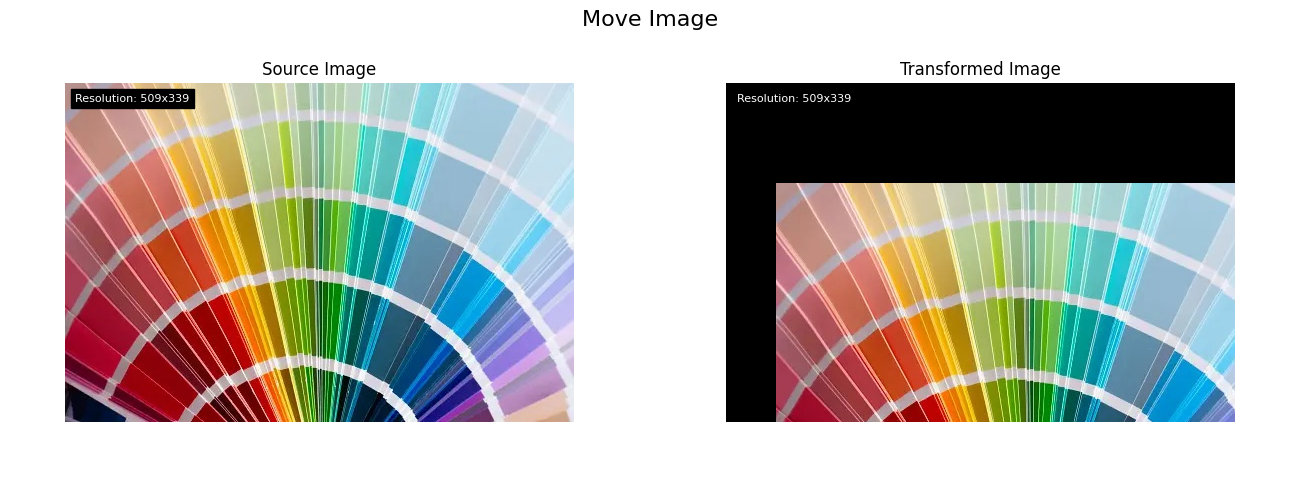
\includegraphics[width=\textwidth]{../results/Move Image.png}
    \caption{Сдвиг изображения}
    \label{fig:move_image}
\end{figure}

% \pagebreak
\subsection{Отражение изображения}

Отражение изображения относительно оси OX можно получить с помощью следующей матрицы преобразования:
\begin{equation}
T = \begin{bmatrix}
    1 & 0 & 0 \\
    0 & -1 & h - 1 \\
    0 & 0 & 1
\end{bmatrix}
\end{equation}
где $h$ -- высота изображения.

Отражение изображения относительно оси OY можно получить с помощью следующей матрицы преобразования:
\begin{equation}
T = \begin{bmatrix}
    -1 & 0 & w - 1 \\
    0 & 1 & 0 \\
    0 & 0 & 1
\end{bmatrix}  
\end{equation}
где $w$ -- ширина изображения.

Использование коэффициентов $h - 1$ и $w - 1$ обусловлено тем, что нам необходимо, чтобы после отражения изображение оставалось в пределах координатной сетки.

Рассмотрим как применить отражение изображения относительно оси OX и OY:

\begin{lstlisting}[style=python_white, caption={Исходный код для отражения изображения относительно оси OX}]
mirror_matrix_x = np.float32([[1, 0, 0], [0, -1, img.shape[0] - 1]])

mirrored_img = apply_matrix_transformations(img, mirror_matrix_x)
show_images(img, mirrored_img, "Mirror Image (x-axis)")
\end{lstlisting}

\begin{figure}[ht]
    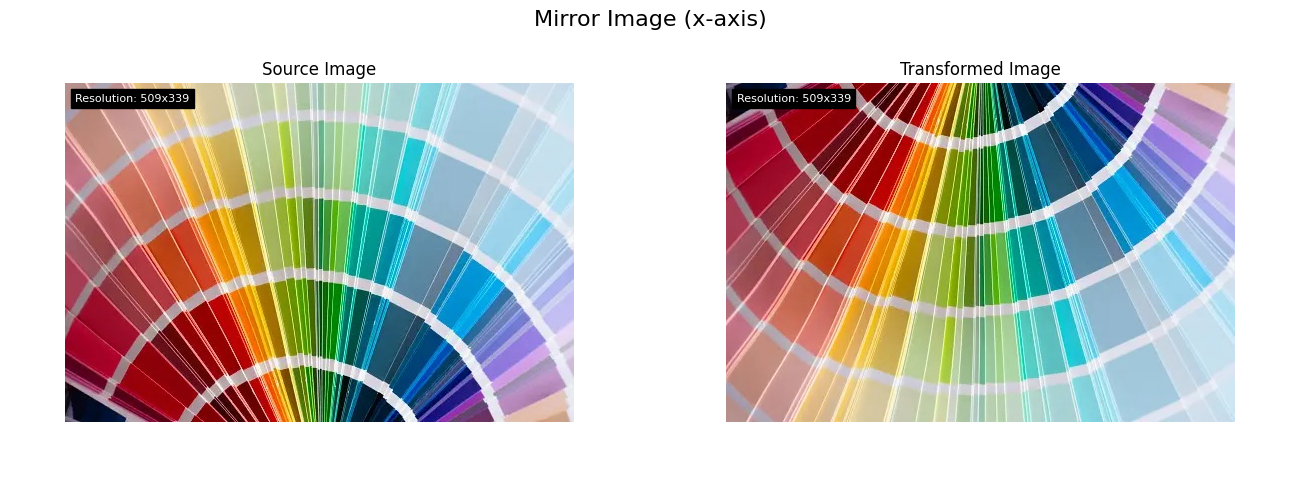
\includegraphics[width=\textwidth]{../results/Mirror Image (x-axis).png}
    \caption{Отражение изображения относительно оси OX}
    \label{fig:mirror_image_x}
\end{figure}

\pagebreak
\begin{lstlisting}[style=python_white, caption={Исходный код для отражения изображения относительно оси OY}]
mirror_matrix_y = np.float32([[-1, 0, img.shape[1] - 1], [0, 1, 0]])

mirrored_img = apply_matrix_transformations(img, mirror_matrix_y)
show_images(img, mirrored_img, "Mirror Image (y-axis)")
\end{lstlisting}

\begin{figure}[ht]
    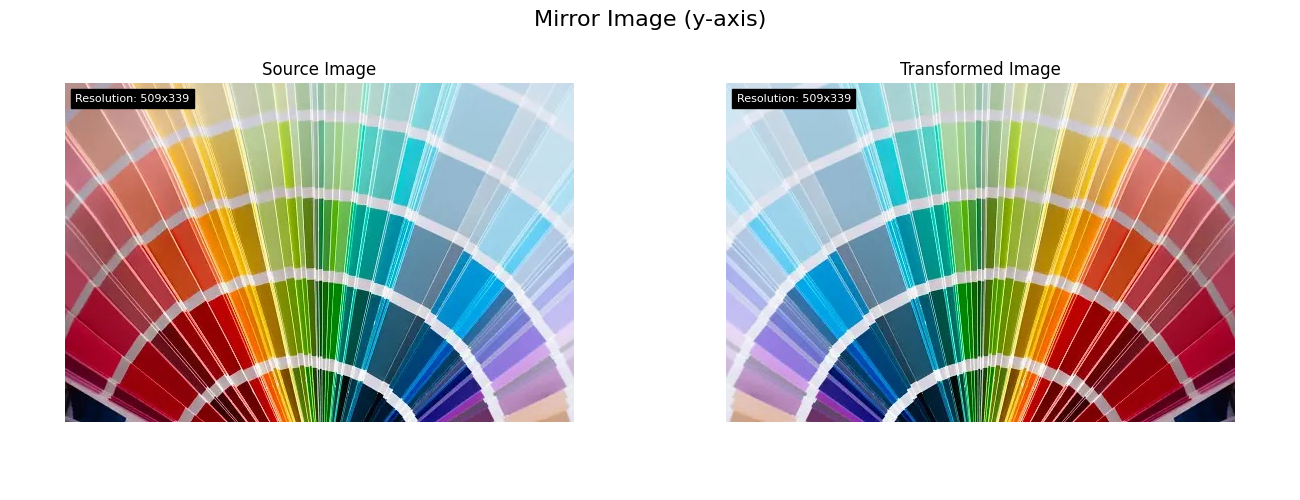
\includegraphics[width=\textwidth]{../results/Mirror Image (y-axis).png}
    \caption{Отражение изображения относительно оси OY}
    \label{fig:mirror_image_Y}
\end{figure}

% \pagebreak
\subsection{Однородное масштабирование изображения}

Для однородного масштабирования изображения на коэффициент $s$ необходимо использовать следующую матрицу преобразования:
\begin{equation}
T = \begin{bmatrix}
    s & 0 & 0 \\
    0 & s & 0 \\
    0 & 0 & 1
\end{bmatrix}
\end{equation}

Рассмотрим как применить однородное масштабирование изображения с коэффициентом 1.5:
\begin{lstlisting}[style=python_white, caption={Исходный код для однородного масштабирования изображения}]
zoom_matrix = np.float32([[1.5, 0, 0], [0, 1.5, 0]])

zoomed_img = apply_matrix_transformations(img, zoom_matrix, (int(img.shape[1] * 1.5), int(img.shape[0] * 1.5)))
show_images(img, zoomed_img, "Zoom Image")
\end{lstlisting}

\begin{figure}[ht]
    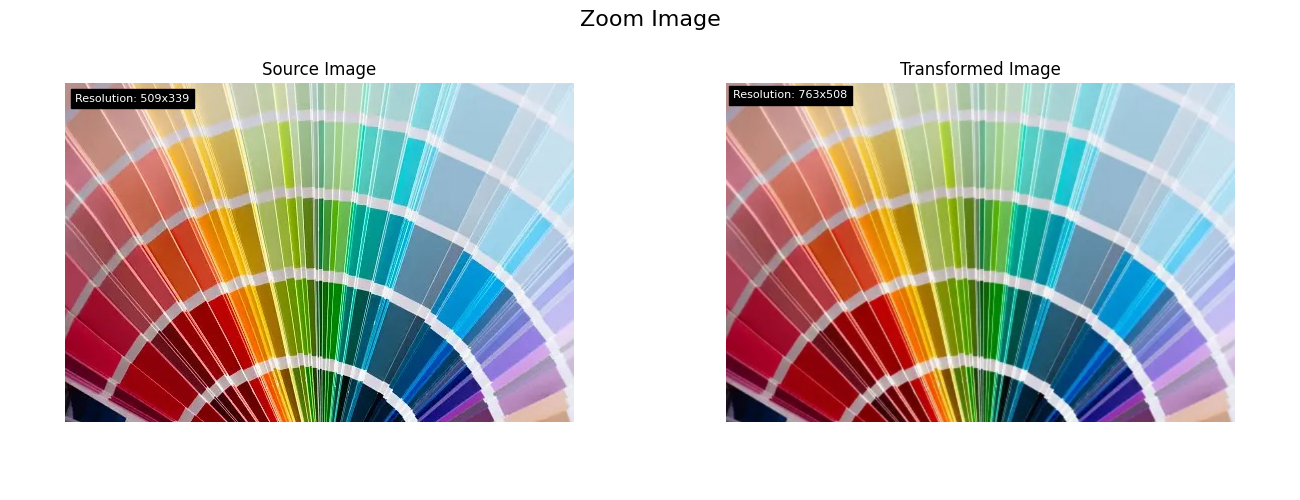
\includegraphics[width=\textwidth]{../results/Zoom Image.png}
    \caption{Однородное масштабирование изображения}
    \label{fig:uniform_scale_image}
\end{figure}

Кроме того, можно использовать функцию \texttt{cv2.resize} из библиотеки OpenCV для однородного масштабирования изображения:
\begin{lstlisting}[style=python_white, caption={Исходный код для однородного масштабирования изображения с использованием библиотеки OpenCV}]
zoomed_img_cv = cv2.resize(img, None, fx=1.5, fy=1.5, interpolation=cv2.INTER_CUBIC)
# None is the size of the output image (None ti use scaling factors), fx and fy are the scale factors
show_images(img, zoomed_img_cv, "Zoom Image (using OpenCV)")
\end{lstlisting}

\begin{figure}[ht]
    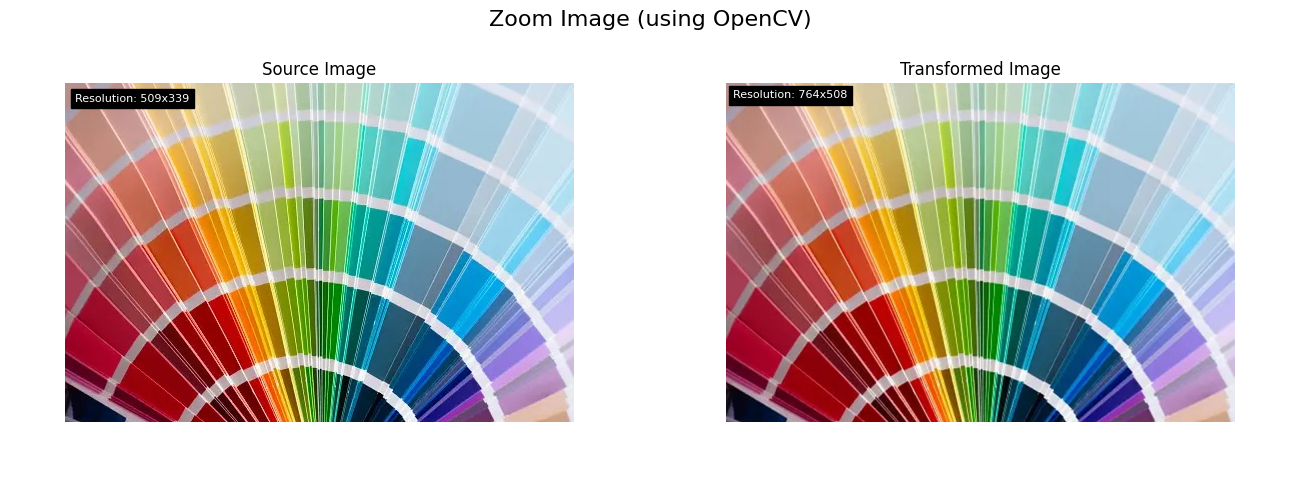
\includegraphics[width=\textwidth]{../results/Zoom Image (using OpenCV).png}
    \caption{Однородное масштабирование изображения с использованием библиотеки OpenCV}
    \label{fig:uniform_scale_image_cv}
\end{figure}

Несмотря на то, что на картинке изображение не изменилось, размер изображения увеличился в 1.5 раза. Это можно увидеть в левом верхнем углу изображения.

% \pagebreak
\subsection{Поворот изображения}

Для поворота изображения на угол $\theta$ необходимо использовать следующую матрицу преобразования:

\begin{equation}
T = \begin{bmatrix}
    \cos(\theta) & -\sin(\theta) & 0 \\
    \sin(\theta) & \cos(\theta) & 0 \\
    0 & 0 & 1
\end{bmatrix}
\end{equation}

Рассмотрим как применить поворот изображения на 10 градусов:
\begin{lstlisting}[style=python_white, caption={Исходный код для поворота изображения}]
angle = np.deg2rad(10)
rotation_matrix = np.float32([[np.cos(angle), -np.sin(angle), 0], [np.sin(angle), np.cos(angle), 0]])

rotated_img = apply_matrix_transformations(img, rotation_matrix)
show_images(img, rotated_img, "Rotate Image")
\end{lstlisting}

\begin{figure}[ht]
    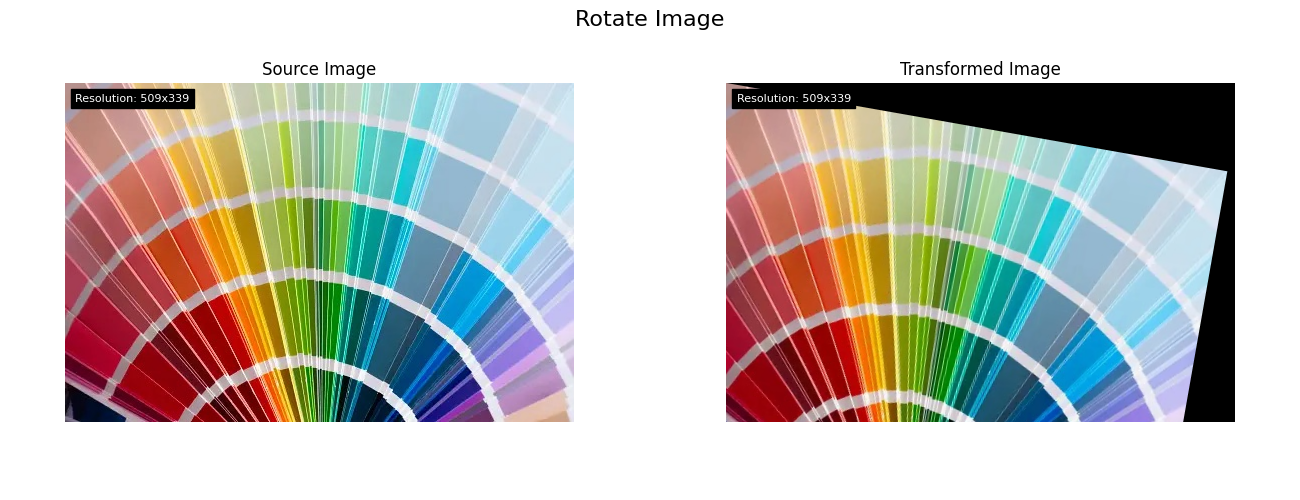
\includegraphics[width=\textwidth]{../results/Rotate Image.png}
    \caption{Поворот изображения}
    \label{fig:rotate_image}
\end{figure}

Видим, что изображения действительно повернулось на 10 градусов против часовой стрелки относительно начала координат, 
которое находится в левом верхнем углу изображения.

Для того, чтобы осуществить поворот изображения относительно определенной точки, необходимо выполнить следующие шаги:

\begin{enumerate}
    \item Переместить изображение так, чтобы точка, относительно которой будет осуществляться поворот, находилась в начале координат
    \item Повернуть изображение относительно начала координат
    \item Переместить изображение обратно
\end{enumerate}

Матрицы для каждого шага будут следующими:
\begin{equation}
T_1 = \begin{bmatrix}
    1 & 0 & -\frac{w}{2} \\
    0 & 1 & -\frac{h}{2} \\
    0 & 0 & 1
\end{bmatrix}
\end{equation}
\begin{equation}
T_2 = \begin{bmatrix}
    \cos(\theta) & -\sin(\theta) & 0 \\
    \sin(\theta) & \cos(\theta) & 0 \\
    0 & 0 & 1
\end{bmatrix}
\end{equation}
\begin{equation}
T_3 = T_1^{-1} = \begin{bmatrix}
    1 & 0 & \frac{w}{2} \\
    0 & 1 & \frac{h}{2} \\
    0 & 0 & 1
\end{bmatrix}
\end{equation}
Применение этих матриц к изображению позволит осуществить поворот изображения относительно центра:
\begin{equation}
    I' = T_3 \times T_2 \times T_1 \times I
\end{equation}

Рассмотрим как применить поворот изображения на 10 градусов относительно центра:
\begin{lstlisting}[style=python_white, caption={Исходный код для поворота изображения с использованием библиотеки OpenCV}]
angle = np.deg2rad(10)
move_to_center_matrix = np.float32([[1, 0, -img.shape[1] / 2], [0, 1, -img.shape[0] / 2], [0, 0, 1]])
rotation_matrix = np.float32([[np.cos(angle), -np.sin(angle), 0], [np.sin(angle), np.cos(angle), 0], [0, 0, 1]])
move_back_matrix = np.float32([[1, 0, img.shape[1] / 2], [0, 1, img.shape[0] / 2], [0, 0, 1]])

transformation_matrix = move_back_matrix @ rotation_matrix @ move_to_center_matrix 
# remove the last row 
transformation_matrix = transformation_matrix[:2, :]

rotated_img = apply_matrix_transformations(img, transformation_matrix)
show_images(img, rotated_img, "Rotate Image (about the center)")
\end{lstlisting}

Кроме того, можно использовать функцию \texttt{cv2.getRotationMatrix2D} из библиотеки OpenCV для поворота изображения относительно центра:
\begin{figure}[ht]
    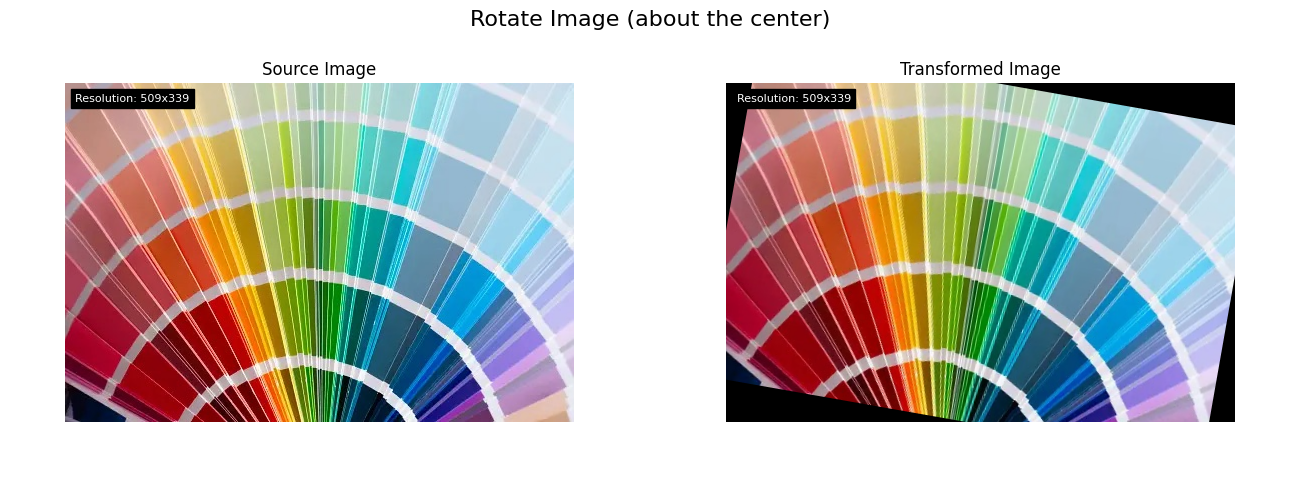
\includegraphics[width=\textwidth]{../results/Rotate Image (about the center).png}
    \caption{Поворот изображения относительно центра}
    \label{fig:rotate_image_center}
\end{figure}

\begin{lstlisting}[style=python_white, caption={Исходный код для поворота изображения относительно центра с использованием библиотеки OpenCV}]
angle = 10
rotation_matrix_cv = cv2.getRotationMatrix2D((img.shape[1] / 2, img.shape[0] / 2), angle, 1)

rotated_img_cv = apply_matrix_transformations(img, rotation_matrix_cv)
show_images(img, rotated_img_cv, "Rotate Image (using OpenCV)")
\end{lstlisting}

\begin{figure}[ht]
    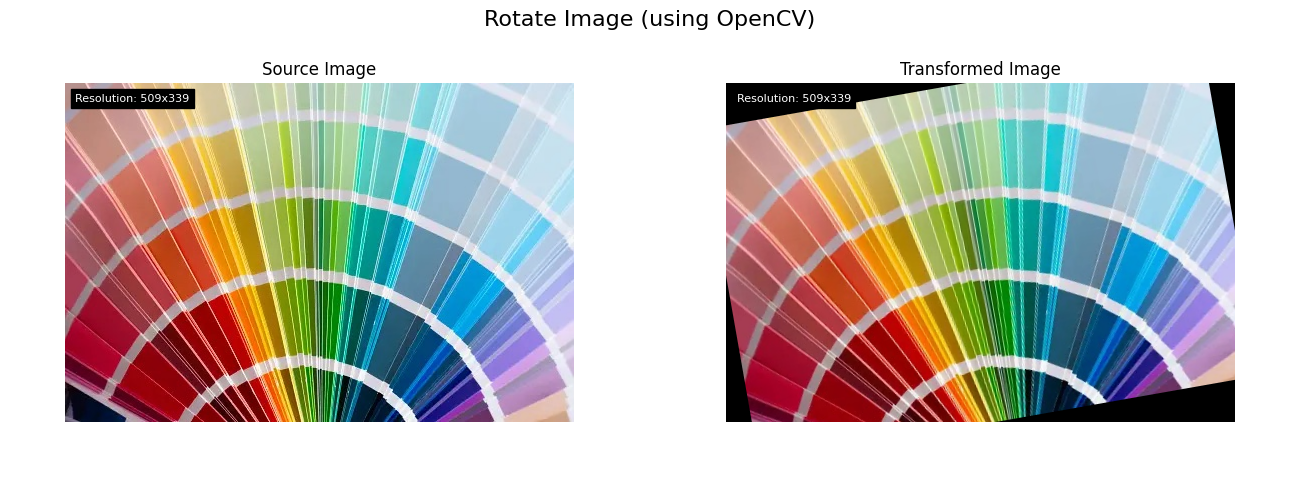
\includegraphics[width=\textwidth]{../results/Rotate Image (using OpenCV).png}
    \caption{Поворот изображения с использованием библиотеки OpenCV}
    \label{fig:rotate_image_cv}
\end{figure}

% \pagebreak
\subsection{Аффинное отображение} 

Аффинное преобразование -- это преобразование, которое сохраняет параллельность прямых, соотношение длин отрезков, лежащих на одной прямой, и углы между пересекающимися прямыми.
Аффинные преобразования являются подмножеством проективных преобразований. 

Для задания аффинного преобразования можно использовать три пары соответствующих точек на исходном и преобразованном изображениях.

Программная реализация аффинного преобразования:
\begin{lstlisting}[style=python_white, caption={Исходный код для аффинного отображения}]
# define the points of the source image
src_points = np.float32([[0, 0], [img.shape[1] - 1, 0], [0, img.shape[0] - 1]])
# define the points of the transformed image
dst_points = np.float32([[50, 50], [img.shape[1] - 1, 0], [0, img.shape[0] - 1]])

affine_matrix = cv2.getAffineTransform(src_points, dst_points)

affine_img = apply_matrix_transformations(img, affine_matrix)
show_images(img, affine_img, "Affine Transformation")
\end{lstlisting}

\begin{figure}[ht]
    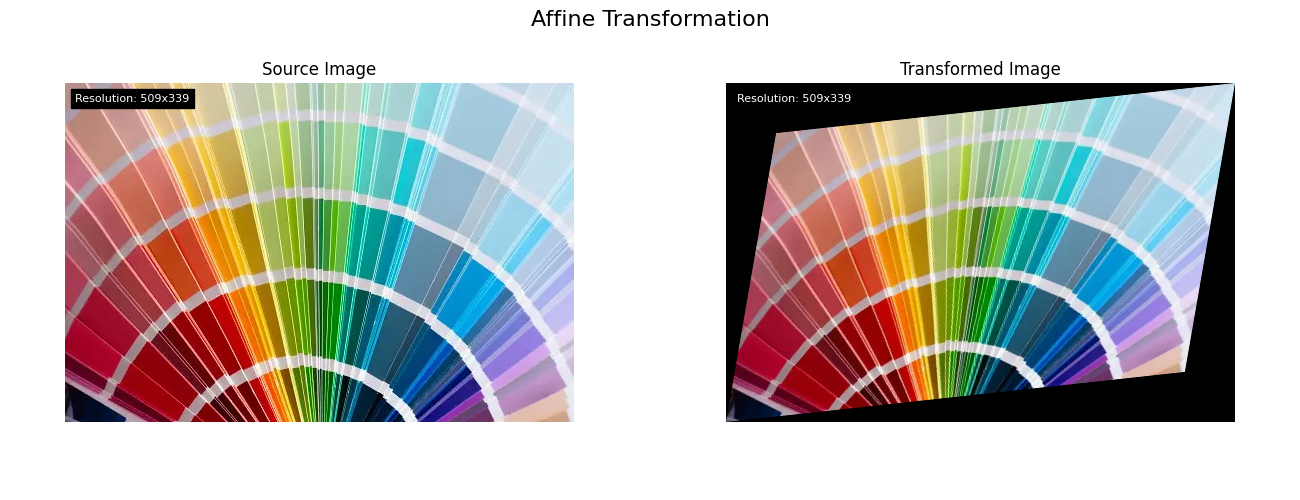
\includegraphics[width=\textwidth]{../results/Affine Transformation.png}
    \caption{Аффинное отображение}
    \label{fig:affine_image}
\end{figure}

% \pagebreak
\subsection{Скос изображения}

Для того, чтобы осуществить скос изображения, необходимо использовать следующую матрицу преобразования:
\begin{equation}
T_1 = \begin{bmatrix}
    1 & \alpha & 0 \\
    0 & 1 & 0 \\
    0 & 0 & 1
\end{bmatrix} \text{или } 
T_2 = \begin{bmatrix}
    1 & 0 & 0 \\
    \beta & 1 & 0 \\
    0 & 0 & 1
\end{bmatrix}
\end{equation}

Рассмотрим как применить скос изображения:
\begin{lstlisting}[style=python_white, caption={Исходный код для скоса изображения}]
shearing_matrix = np.float32([[1, 0, 0], [0.2, 1, 0]])

sheared_img = apply_matrix_transformations(img, shearing_matrix)
show_images(img, sheared_img, "Shearing Transformation")
\end{lstlisting}

\begin{figure}[ht]
    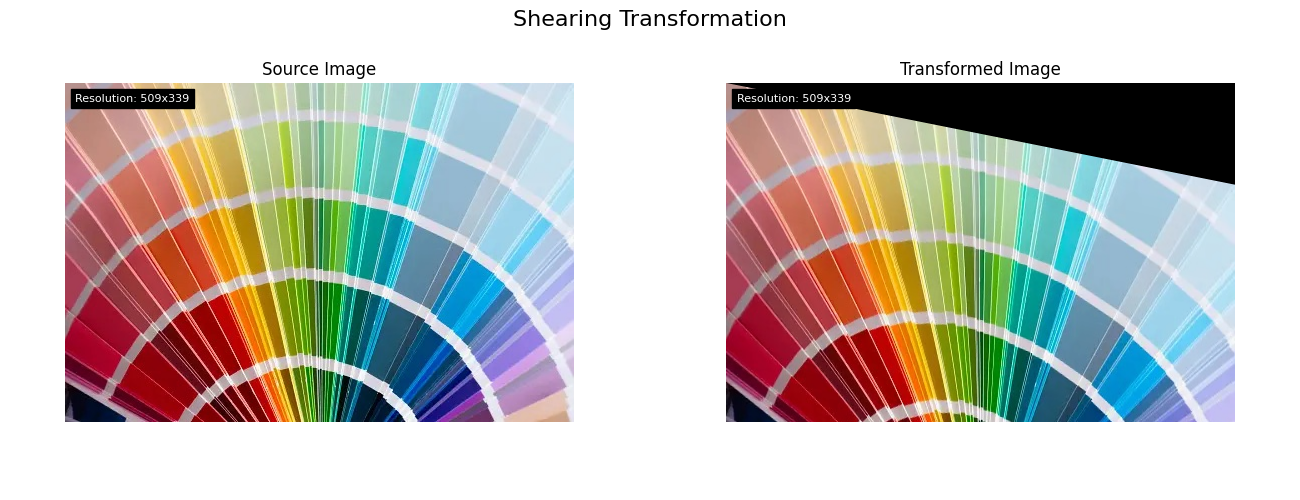
\includegraphics[width=\textwidth]{../results/Shearing Transformation.png}
    \caption{Скос изображения}
    \label{fig:sheared_image}
\end{figure}

\pagebreak
\subsection{Кусочно-линейное преобразование}

Кусочно-линейное преобразование -- это преобразование, при котором изображение разбивает на части, и каждая часть преобразуется отдельно.
Например, можно рассмотреть преобразование, которое левую часть оставляет без изменений, а правую часть растягивает в 4 раза.
\begin{lstlisting}[style=python_white, caption={Исходный код для кусочно-линейного преобразования}]
stretch = 4
piecewise_linear_matrix = np.float32([[stretch, 0, 0], [0, 1, 0]])

piecewise_linear_img = img.copy()
piecewise_linear_img[:, img.shape[1] // 2:] = apply_matrix_transformations(img[:, img.shape[1] // 2:], piecewise_linear_matrix)

show_images(img, piecewise_linear_img, "Piecewise Linear Transformation")
\end{lstlisting}

\begin{figure}[ht]
    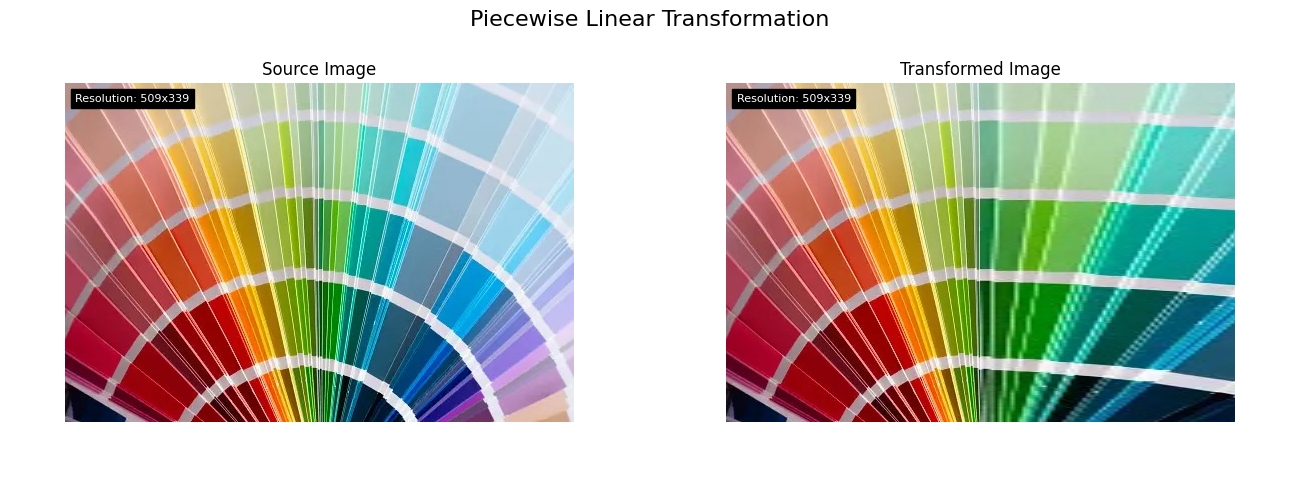
\includegraphics[width=\textwidth]{../results/Piecewise Linear Transformation.png}
    \caption{Кусочно-линейное преобразование}
    \label{fig:piecewise_linear_image}
\end{figure}

% \pagebreak
\section{Нелинейные преобразования}

В реальности необходимо применять не только линейные преобразования, но и нелинейные.
Например, для коррекции дисторсии, которая вызывается несовершенством оптики, необходимо использовать нелинейные преобразования.

\subsection{Проекционное отображение}
Проекционное отображение -- это отображение, которое оставляет прямые линии прямыми, но геометрия изображения может быть искажена, так как 
данное отображение не сохраняет углы между прямыми.

Матрица для проекционного отображения в общем виде выглядит следующим образом:

\begin{equation}
T = \begin{bmatrix}
    A & B & E \\
    C & D & F \\
    G & H & K \\
\end{bmatrix}
\end{equation}
где $A, B, C, D$ -- коэффициенты, которые определяют проекционное отображение, $E, F$~--~коэффициенты сдвига, $G, H$~--~коэффициенты, которые определяют проекционное отображение, $K$~--~коэффициент масштабирования.

Рассмотрим как применить проективное отображение:
\begin{lstlisting}[style=python_white, caption={Исходный код для проективного отображения}]
projective_matrix = np.float32([[1.1, 0.35, 0], [0.2, 1.1, 0], [0.00075, 0.0005, 1]])

projective_img = apply_perspective_transformations(img, projective_matrix)
show_images(img, projective_img, "Projective Transformation")
\end{lstlisting}

\begin{figure}[ht]
    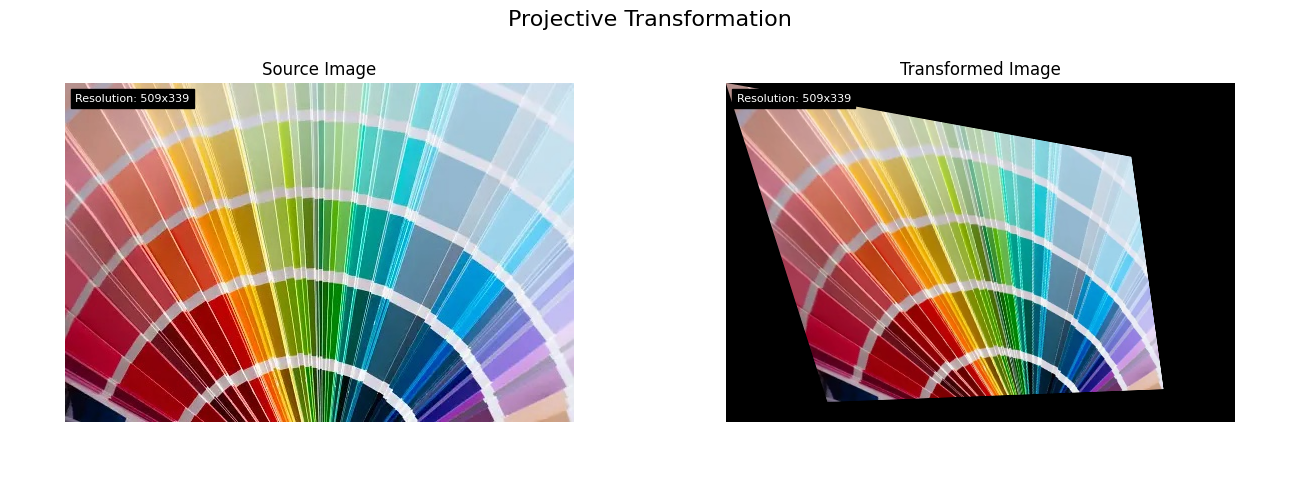
\includegraphics[width=\textwidth]{../results/Projective Transformation.png}
    \caption{Проективное отображение}
    \label{fig:projective_image}
\end{figure}

% \pagebreak
\subsection{Полиномиальное преобразование}

Полиномиальное преобразование -- это отображение исходного изображения на преобразованное с использованием полиномиальной функции.

Полиномиальное преобразование второго порядка выглядит следующим образом:
\begin{equation}
\begin{cases}
    x' = a_0 + a_1x + a_2y + a_3x^2 + a_4xy + a_5y^2\\
    y' = b_0 + b_1x + b_2y + b_3x^2 + b_4xy + b_5y^2
\end{cases}
\end{equation}


\begin{lstlisting}[style=python_white, caption={Исходный код для полиномиального преобразования}]
polynomial_matrix = np.float32([[0, 0], [1, 0], [0, 1], [0.00001, 0], [0.002, 0], [0.001, 0]])

polynomial_img = np.zeros_like(img)
x, y = np.meshgrid(np.arange(img.shape[1]), np.arange(img.shape[0]))

# calculate the new coordinates
xnew = np.round(polynomial_matrix[0, 0] + polynomial_matrix[1, 0] * x + polynomial_matrix[2, 0] * y + polynomial_matrix[3, 0] * x**2 + polynomial_matrix[4, 0] * x * y + polynomial_matrix[5, 0] * y**2).astype(np.float32)
ynew = np.round(polynomial_matrix[0, 1] + polynomial_matrix[1, 1] * x + polynomial_matrix[2, 1] * y + polynomial_matrix[3, 1] * x**2 + polynomial_matrix[4, 1] * x * y + polynomial_matrix[5, 1] * y**2).astype(np.float32)

# calculate mask for valid coordinates
mask = np.logical_and(np.logical_and(xnew >= 0, xnew < img.shape[1]), np.logical_and(ynew >= 0, ynew < img.shape[0]))

# apply the transformation
if img.ndim == 2:
    polynomial_img[ynew[mask].astype(int), xnew[mask].astype(int)] = img[y[mask], x[mask]]
else:
    polynomial_img[ynew[mask].astype(int), xnew[mask].astype(int), :] = img[y[mask], x[mask], :]

show_images(img, polynomial_img, "Polynomial Transformation")
\end{lstlisting}

\begin{figure}[ht]
    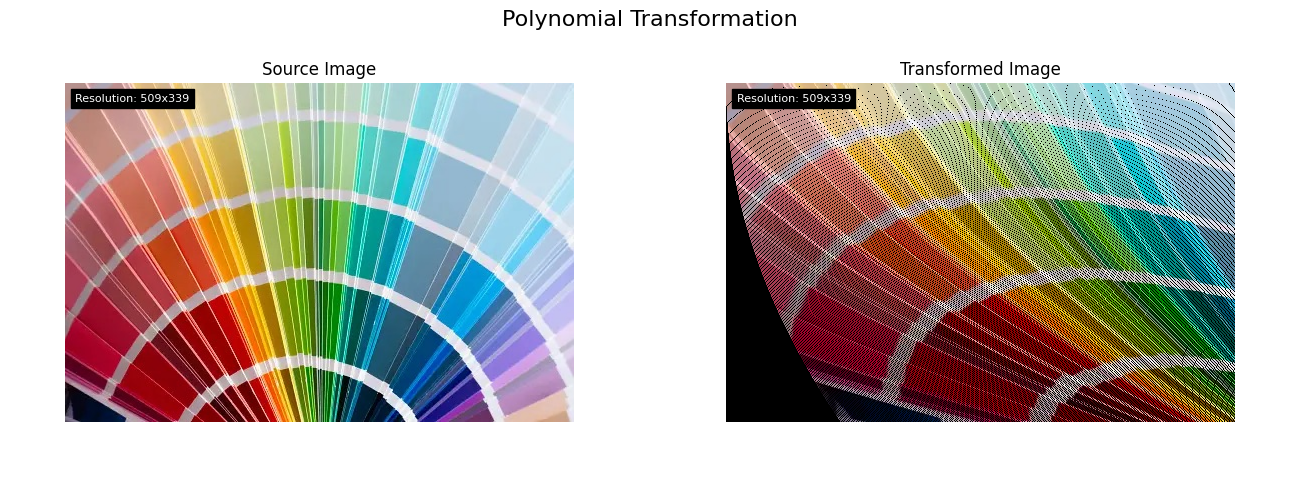
\includegraphics[width=\textwidth]{../results/Polynomial Transformation.png}
    \caption{Полиномиальное преобразование}
    \label{fig:polynomial_image}
\end{figure}

Видим, что на изображении появились артефакты, так как не все пиксели были заполнены. Это связано с тем, что при применении полиномиального преобразования
цвета пикселей могут быть не определены для некоторых координат, и в таком случае необходимо использовать интерполяцию.

% \pagebreak
\subsection{Синусоидальное искажение}

Еще одним примером нелинейного преобразования может быть искажение изображения по гармоническому закону.

\begin{lstlisting}[style=python_white, caption={Исходный код для синусоидального искажения}]
u, v = np.meshgrid(np.arange(img.shape[1]), np.arange(img.shape[0]))
v = v + 15 * np.sin(2 * np.pi * u / 90)

img_sinusoidal = cv2.remap(img, u.astype(np.float32), v.astype(np.float32), cv2.INTER_LINEAR)

show_images(img, img_sinusoidal, "Sinusoidal Transformation")
\end{lstlisting}

\begin{figure}[ht]
    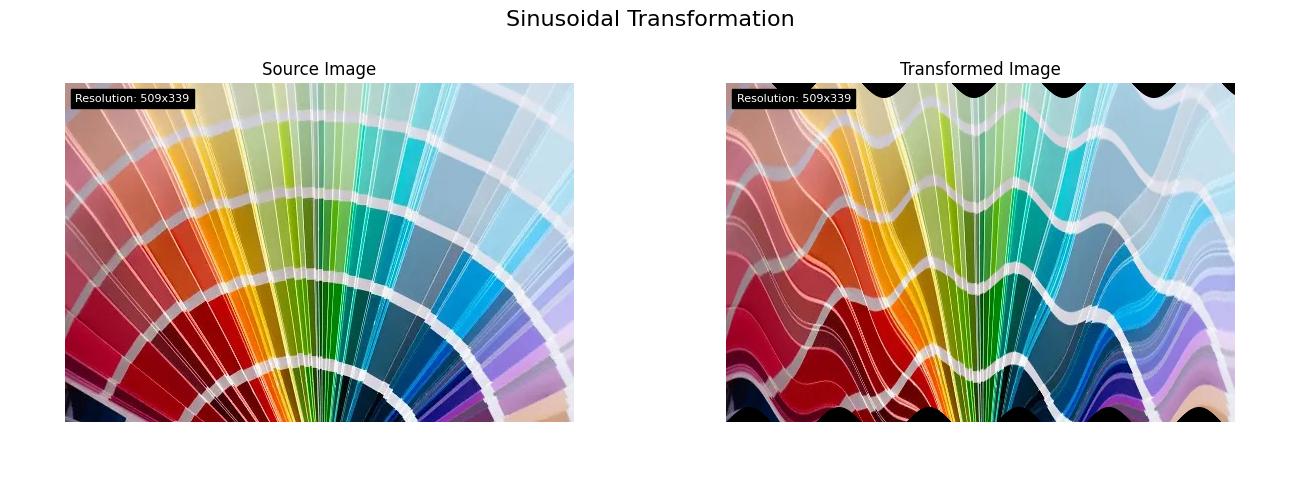
\includegraphics[width=\textwidth]{../results/Sinusoidal Transformation.png}
    \caption{Синусоидальное искажение}
    \label{fig:sinusoidal_image}
\end{figure}

% \pagebreak
\subsection{Коррекция дисторсии}

При формировании изображения оптической системой камеры, на нем может возникнуть дисторсия, которая вызвана несовершенством оптики.
\textbf{Дисторсия} -- это оптическое искажение, которое искривляет прямые линии на изображении.

\begin{lstlisting}[style=python_white, caption={Исходный код для коррекции бочкообразной дисторсии}]
img_distortion_corrected = distortion_correction(img, lambda r: r + 0.16 * r ** 3 + 0.1 * r ** 5)
show_images(img, img_distortion_corrected, "Distortion Correction (barrel)")
\end{lstlisting}

\begin{figure}[ht]
    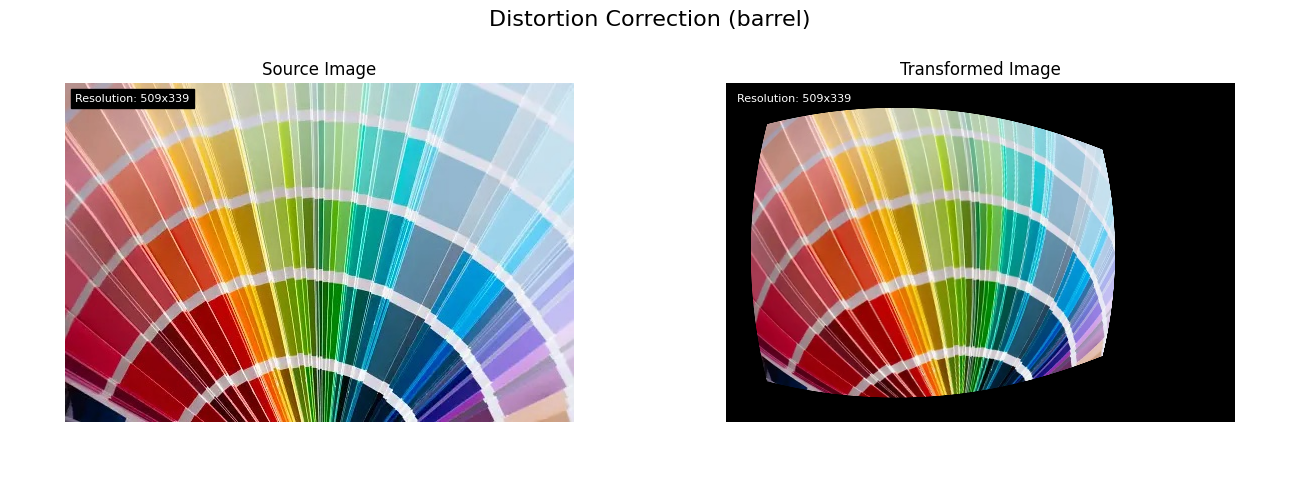
\includegraphics[width=\textwidth]{../results/Distortion Correction (barrel).png}
    \caption{Коррекция дисторсии (бочка)}
    \label{fig:distortion_correction_barrel}
\end{figure}

\begin{lstlisting}[style=python_white, caption={Исходный код для коррекции подушкообразной дисторсии}]
img_distortion_corrected = distortion_correction(img, lambda r: r - 0.3 * r ** 2)
show_images(img, img_distortion_corrected, "Distortion Correction (pincushion)")
\end{lstlisting}

\begin{figure}[ht]
    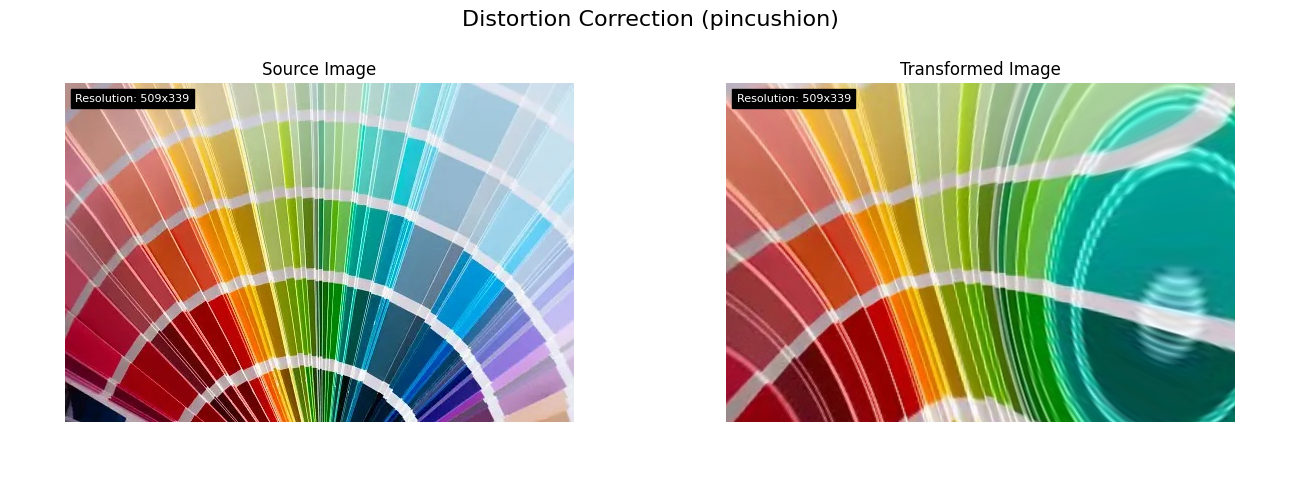
\includegraphics[width=\textwidth]{../results/Distortion Correction (pincushion).png}
    \caption{Коррекция дисторсии (подушка)}
    \label{fig:distortion_correction_pincushion}
\end{figure}

\pagebreak
\section{Сшивка изображений}

Сшивка изображений -- это процесс объединения двух или более изображений в одно.
Для того, чтобы осуществить сшивку изображений, необходимо найти общие точки на изображениях, и на основе этих точек осуществить сшивку, 
перейдя от системы координат одного изображения к системе координат другого изображения.

Посмотрим на два изображения, которые необходимо сшить:

\begin{figure}[ht]
    \centering
    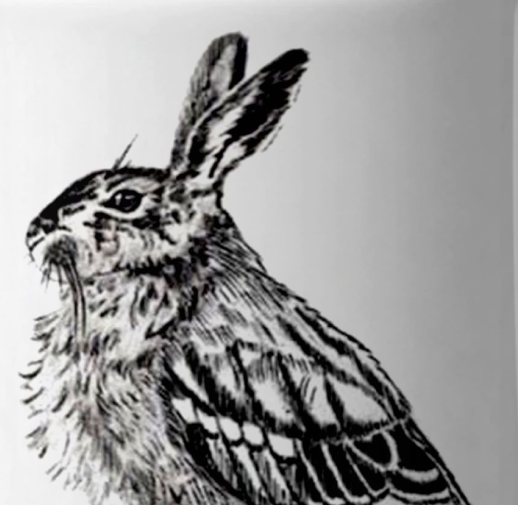
\includegraphics[width=0.4\textwidth]{../zaebushek_top.png}
    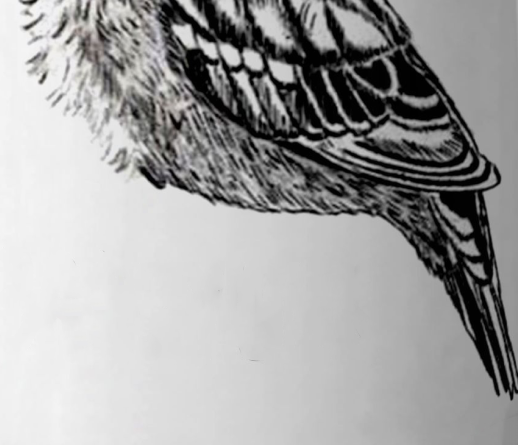
\includegraphics[width=0.40\textwidth]{../zaebushek_bttm.png}
    \caption{Изображения для сшивки}
    \label{fig:stitch_images}
\end{figure}

На рисунке \ref{fig:stitch_images} видно, что изображения имеют общую часть, и на основе этой части можно осуществить сшивку.

Посмотрим на несколько способов сшивки изображений:

\begin{lstlisting}[style=python_white, caption={Исходный код для сшивки изображений}]
template_size = 20

template = img_top[-template_size:, :, :]

res = cv2.matchTemplate(img_bttm, template, cv2.TM_CCOEFF)
min_val, max_val, min_loc, max_loc = cv2.minMaxLoc(res)

result_img = np.zeros((img_bttm.shape[0] + img_top.shape[0] - max_loc[1] - template_size, img_top.shape[1], img_top.shape[2]), dtype=np.uint8)
result_img[:img_top.shape[0], :, :] = img_top
result_img[img_top.shape[0]:, :, :] = img_bttm[max_loc[1] + template_size:, :, :]

show_images(img_source, result_img, "Merged Images")
\end{lstlisting}

\begin{figure}[ht]
    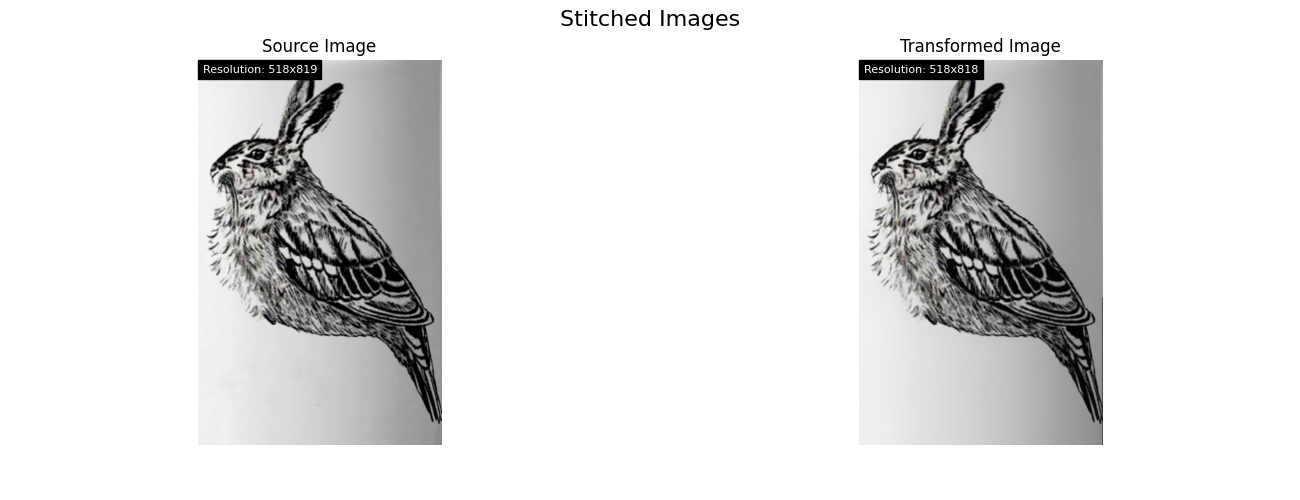
\includegraphics[width=\textwidth]{../results/Stitched Images.png}
    \caption{Сшивка изображений}
    \label{fig:stitched_images}
\end{figure}


\begin{lstlisting}[style=python_white, caption={Исходный код для сшивки изображений с использованием библиотеки OpenCV}]
stitcher = cv2.Stitcher.create(cv2.Stitcher_SCANS)
status, result_img = stitcher.stitch((img_top, img_bttm))

if status == 0:
    show_images(img_source, result_img, "Stitched Images (using OpenCV)")
else:
    print("Images could not be stitched")
\end{lstlisting}

\begin{figure}[ht]
    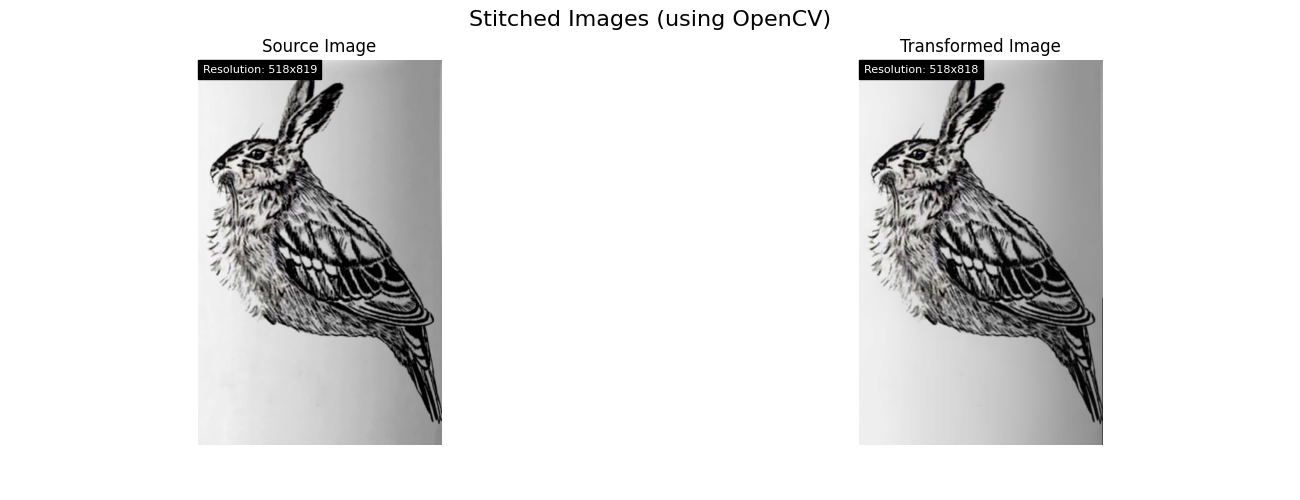
\includegraphics[width=\textwidth]{../results/Stitched Images (using OpenCV).png}
    \caption{Сшивка изображений с использованием библиотеки OpenCV}
    \label{fig:stitched_images_cv}
\end{figure}

Видим, что при использовании каждого из методов изображения были успешно сшиты.

\pagebreak
\section{Выводы}
В процессе выполнения лабораторной работы мы освоили основные виды отображений и использовали различные геометрические преобразования, попробовали скорректировать оптические искажения. Мы научились применять эти преобразования с использованием языка Python и функций \texttt{affine2d(), cv2.warpAffine(), flip(), getRotationMatrix2D()} и других. 

Также смогли оценить качество полученных изображений и убедиться, что геометрические преобразования позволяют улучшать их визуальное восприятие

\section{Ответы на вопросы}

\newcounter{question}
\setcounter{question}{0}

\newcommand{\question}[1]{\item[Q\refstepcounter{question}\thequestion.] #1}
\newcommand{\answer}[1]{\item[A\thequestion.] #1}

\begin{itemize}

\question{Каким образом можно выполнить поворот изображения, не используя матрицу поворота?}
\answer{Можно воспользоваться функцией \texttt{rotate()} в библиотеке OpenCV, которая используется как раз для поворота изображения. Метод \texttt{rotate()} принимает угол вращения в градусах в качестве аргумента. 
По умолчанию размер готового изображения равен размеру исходного изображения, и части повернутого изображения, которые выходят за пределы исходного размера, отсекаются.
Если мы хотим, чтобы повернутое изображение полностью удовлетворяло нашим требованиям, мы можем установить параметр \texttt{expand} в \texttt{True}.}

\question{Какое минимальное количество соответствующих пар точек необходимо задать на исходном и искаженном изображениях, если порядок преобразования $n = 4$?}
\answer{Число минимально необходимых пар точек вычисляется по формуле:

$t_{min} = ((n+1)\cdot(n+2))/2$, 
где $n$ - порядок преобразования. Следовательно, при $n = 4$ нам потребуется минимум 15 пар точек.}

\question{После геометрического преобразования изображения могут появиться пиксели с неопределенными значениями интенсивности. С чем это связано и как решается данная проблема?}
\answer{При геометрическом преобразовании, когда мы изменяем размер, поворачиваем или искажаем изображение, пиксели перемещаются и могут попасть в пространство между исходными пикселями. Это приводит к неопределенным значениям интенсивности. 
Для решения этой проблемы используется \textit{интерполяция}. Она позволяет вычислить значения для неопределенных пикселей на основе соседних известных пикселей.
Существует функция \texttt{affine2d()}, которая создает матрицу преобразования. Ее параметры задают одинаковые координаты для исходного и преобразованного изображений, а также метод интерполяции для неопределенных пикселей.}

\end{itemize}

